\chapter{Conservation Laws}

% ============ Problem 1 ============ %

\begin{problem}
{
A particle of mass $m$ moving with velocity $\mathbf{v}_1$ leaves a half-space in which its potential energy is a constant $U_1$ and enters another in which its potential energy is a different constant $U_2$. Determine the change in the direction of motion of the particle.
}
{
The potential energy only depend on the co-ordinate perpendicular to the plane separating the half-space. Thus, the component of the momentum in that plane is conserved. Denoting by $\theta_1$ and $\theta_2$ the angles between the normal to the plane and the velocities $v_1$ and $v_2$ of the particle before and after passing the plane, we have
\begin{align*}
    & P_1 \sin{\theta_1} = P_2 \sin{\theta_2} \\
    \Rightarrow & v_1 \sin{\theta_1} = v_2 \sin{\theta_2} \\
    \Rightarrow & \frac{\sin{\theta_1}}{\sin{\theta_2}} = \frac{v_2}{v_1} . \numberthis \label{C2P1_P}
\end{align*}
The potential energy of the system is also independent of time, therefore the energy of the particle is conserved. Posing $E_1 = T_1 + U_1$ and $E_2 = T_2 + U_2$ as the energy of the particle before and after passing the plane, the law of conservation of energy requires
\begin{align*}
    &E_1 = E_2 \\
    \Rightarrow & T_1 + U_1 = T_2 + U_2 \\
    \Rightarrow &\frac{1}{2} m v_1^2 + U_1 = \frac{1}{2} m v_2^2 + U_2 \\
    \Rightarrow & v_2^2 = v_1^2 + \frac{2}{m}(U_1-U_2). \numberthis \label{C2P1_E}
\end{align*}
By substituting \eqref{C2P1_E} in the square of \eqref{C2P1_P}, we get
\begin{equation*}
    \left( \frac{\sin{\theta_1}}{\sin{\theta_2}} \right)^2 = \frac{v_1^2 + \frac{2}{m}(U_1-U_2)}{v_1^2}.
\end{equation*}
After taking the square root, the result is  
}
{
\begin{equation*}
    \frac{\sin{\theta_1}}{\sin{\theta_2}} = \sqrt{1 + \frac{2}{mv_1^2}(U_1-U_2)}
\end{equation*}
}
\end{problem}

% ============ Problem 2 ============ %

\begin{problem}
{
Find the law of transformation of the action $S$ from one inertial frame to another.
}
{
The Lagrangian $L$ and $L'$ of a mechanical system in two inertial frames of reference $K$ and $K'$ are respectively
\begin{equation*}
    L = T - U = \frac{1}{2} \sum_a m_a v_a^2 - U
\end{equation*}
and
\begin{equation*}
    L' = T' - U = \frac{1}{2} \sum_a m_a v_a^{'2} - U.
\end{equation*}
If the frame $K'$ moves with velocity $\mathbf{V}$ relative to the frame $K$, the velocities of the particles of the mechanical system relative to the two frames are related by $\mathbf{v}_a = \mathbf{v}_a' + \mathbf{V}$. We can now express the relation of the Lagrangian of the system in the two frames by
\begin{align*}
    L &= \frac{1}{2} \sum_a m_a (\mathbf{v}_a' + \mathbf{V})^2 - U \\ 
    &= \frac{1}{2} V^2 \sum_a m_a + \mathbf{V} \cdot \sum_a m_a \mathbf{v}_a' + \frac{1}{2} \sum_a m_a v_a^{'2} - U \\
    &= L' + \mathbf{V} \cdot \mathbf{P}' + \frac{1}{2} \mu V^2 . \numberthis \label{C3P2_L}
\end{align*}
Integrating \eqref{C3P2_L} with respect to time, we obtain
\begin{align*}
    S &= \int L dt \\
    &= S' + \int \left( \mathbf{V} \cdot \mathbf{P}' \right)dt + \frac{1}{2} \mu V^2 t \\
    &= S' + \mathbf{V} \cdot \int \sum_a m_a \mathbf{v}_a' dt + \frac{1}{2} \mu V^2 t \\
    &= S' + \mathbf{V} \cdot \sum_a m_a \mathbf{r}_a' + \frac{1}{2} \mu V^2 t .
\end{align*}
The law of transformation of the action $S$ is then
}
{
\begin{equation*}
    S = S' + \mu \mathbf{V} \cdot \mathbf{R}' + \frac{1}{2} \mu V^2 t
\end{equation*}
}
\end{problem}

% ============ Problem 3 ============ %

\begin{problem}
{
Obtain the expressions for the Cartesian components and the magnitude of the angular momentum of a particle in cylindrical co-ordinates $r,\phi,z$.
}
{
The Cartesian components of the angular momentum are simply
\begin{equation*}
    \mathbf{M} = \mathbf{r} \times \mathbf{p} = \begin{bmatrix} x \\ y \\ z \end{bmatrix} \times m \begin{bmatrix} \Dot{x} \\ \Dot{y} \\ \Dot{z} \end{bmatrix} = m \begin{bmatrix} y \Dot{z} - z \Dot{y} \\ z \Dot{x} - x \Dot{z} \\ x \Dot{y} - y \Dot{x} \end{bmatrix} . \numberthis \label{C3P3_M}
\end{equation*}
In cylindrical co-ordinates, the Cartesian components are expressed by
\begin{equation*}
    \begin{bmatrix} x \\ y \\ z \end{bmatrix} = \begin{bmatrix} r \cos{\phi} \\ r \sin{\phi} \\ z \end{bmatrix}
\end{equation*}
and
\begin{equation*}
    \begin{bmatrix} \Dot{x} \\ \Dot{y} \\ \Dot{z} \end{bmatrix} = \begin{bmatrix} \Dot{r}\cos{\phi} - r\Dot{\phi}\sin{\phi} \\ \Dot{r}\sin{\phi} + r\Dot{\phi}\cos{\phi} \\ \Dot{z} \end{bmatrix}.
\end{equation*}
By substituting those in \eqref{C3P3_M}, we get
\begin{align*}
    \mathbf{M} &= m \begin{bmatrix} y \Dot{z} - z \Dot{y} \\ z \Dot{x} - x \Dot{z} \\ x \Dot{y} - y \Dot{x} \end{bmatrix} \\
    &= m \begin{bmatrix} (r\Dot{z} - z\Dot{r})\sin{\phi} - rz\Dot{\phi}\cos{\phi} \\ -(r\Dot{z} - z\Dot{r})\cos{\phi} - rz\Dot{\phi}\sin{\phi} \\ r^2\Dot{\phi} \end{bmatrix} . \numberthis \label{C3P3_M2}
\end{align*}
By taking the magnitude of \eqref{C3P3_M2}, we finally get
}
{
\begin{align*}
    M_x &= m(r\Dot{z} - z\Dot{r})\sin{\phi} - mrz\Dot{\phi}\cos{\phi} \\
    M_y &= -m(r\Dot{z} - z\Dot{r})\cos{\phi} - mrz\Dot{\phi}\sin{\phi} \\
    M_z &= mr^2\Dot{\phi} \\
    M^2 &= m^2r^2\Dot{\phi}^2(r^2 + z^2) + m^2(r\Dot{z} - z\Dot{r})^2
\end{align*}
}
\end{problem}

% ============ Problem 4 ============ %

\begin{problem}
{
Obtain the expressions for the Cartesian components and the magnitude of the angular momentum of a particle in spherical co-ordinates $r,\theta,\phi$.
}
{
In spherical co-ordinates, the Cartesian components are expressed by
\begin{equation*}
    \begin{bmatrix} x \\ y \\ z \end{bmatrix} = \begin{bmatrix} r \sin{\phi} \cos{\theta} \\ r \sin{\phi} \sin{\theta} \\ r \cos{\phi} \end{bmatrix}
\end{equation*}
and
\begin{equation*}
    \begin{bmatrix} \Dot{x} \\ \Dot{y} \\ \Dot{z} \end{bmatrix} = \begin{bmatrix} \Dot{r}\sin{\phi}\cos{\theta} + r\Dot{\phi}\cos{\phi}\cos{\theta} - r\Dot{\theta}\sin{\phi}\sin{\theta} \\ \Dot{r}\sin{\phi}\sin{\theta} + r\Dot{\phi}\cos{\phi}\sin{\theta} + r\Dot{\theta}\sin{\phi}\cos{\theta} \\ \Dot{r}\cos{\phi} + r\sin{\phi} \end{bmatrix}.
\end{equation*}
By substituting those in \eqref{C3P3_M}, we get
\begin{align*}
    \mathbf{M} &= m \begin{bmatrix} y \Dot{z} - z \Dot{y} \\ z \Dot{x} - x \Dot{z} \\ x \Dot{y} - y \Dot{x} \end{bmatrix} \\
    &= m \begin{bmatrix} -r^2(\Dot{\theta}\sin{\phi} + \Dot{\phi}\sin{\theta}\cos{\theta}\cos{\phi}) \\ r^2(\Dot{\theta}\cos{\phi} - \Dot{\phi}\sin{\theta}\cos{\theta}\sin{\phi}) \\ r^2\Dot{\phi}\sin^2{\theta} \end{bmatrix} . \numberthis \label{C3P3_M3}
\end{align*}
By taking the magnitude of \eqref{C3P3_M3}, we finally get
}
{
\begin{align*}
    M_x &= -mr^2(\Dot{\theta}\sin{\phi} + \Dot{\phi}\sin{\theta}\cos{\theta}\cos{\phi}) \\
    M_y &= mr^2(\Dot{\theta}\cos{\phi} - \Dot{\phi}\sin{\theta}\cos{\theta}\sin{\phi}) \\
    M_z &= mr^2\Dot{\phi}\sin^2{\theta} \\
    M^2 &= m^2r^4(\Dot{\theta}^2 + \Dot{\phi}^2\sin^2{\theta})
\end{align*}
}
\end{problem}

% ============ Problem 5 ============ %

\begin{problem}
{
Which components of momentum $\mathbf{P}$ and angular momentum $\mathbf{M}$ are conserved in motion in the following fields ?
}{}{}
\end{problem}
\begin{subproblem}
{
The field of an infinite homogeneous plane.
}
{
solution
\begin{figure}[H]
    \centering
    \includegraphics[page=5]{Figures/tikzpics.pdf}
\end{figure}
}
{
answer
}
\end{subproblem}

\begin{subproblem}
{
The field of an infinite homogeneous cylinder.
}
{
solution
}
{
answer
}
\end{subproblem}

\begin{subproblem}
{
The field of an infinite homogeneous prism.
}
{
solution
}
{
answer
}
\end{subproblem}

\begin{subproblem}
{
The field of two points.
}
{
solution
}
{
answer
}
\end{subproblem}

\begin{subproblem}
{
The field of an infinite homogeneous half-plane.
}
{
solution
}
{
answer
}
\end{subproblem}

\begin{subproblem}
{
The field of a homogeneous cone.
}
{
solution
}
{
answer
}
\end{subproblem}

\begin{subproblem}
{
The field of a homogeneous circular torus.
}
{
solution
}
{
answer
}
\end{subproblem}

\begin{subproblem}
{
The field of an infinite homogeneous cylindrical helix.
}
{
solution
}
{
answer
}
\end{subproblem}

% ============ Problem 6 ============ %

\begin{problem}
{
Find the ratio of the times in the same path for particles having different masses but the same potential energy.
}
{
If the two particles have the same path, then the ratio of linear dimension is
\begin{equation} \label{C3P1_l}
    \frac{l'}{l} = \alpha = 1.
\end{equation}
We can define the ratio of time and mass by
\begin{equation*}
    \frac{t'}{t} = \beta
\end{equation*}
and
\begin{equation*}
    \frac{m'}{m} = \gamma .
\end{equation*}
Then, the ratio of kinetic energy is 
\begin{equation*}
    \frac{T'}{T} = \frac{m' \mathbf{v}'}{m \mathbf{v}} = \frac{m'}{m} \left( \frac{\mathbf{dr}'}{\mathbf{dr}} \frac{dt}{dt'} \right)^2 = \frac{\gamma \alpha^2}{\beta^2}.
\end{equation*}
To leave the equation of motion unaltered, the ratio of the kinetic energy and the potential energy must be the same, \ie,
\begin{align*}
    \frac{U'}{U} &= \frac{T'}{T} \\
    \Rightarrow \alpha^k &=  \frac{\gamma \alpha^2}{\beta^2}.
\end{align*}
Using \eqref{C3P1_l}, we get
\begin{align*}
    1 &= \frac{\gamma}{\beta^2} \\
    \Rightarrow \beta &= \sqrt{\gamma}.
\end{align*}
The ratio of the times is then
}
{
\begin{equation*}
    \frac{t'}{t} = \sqrt{\frac{m'}{m}}
\end{equation*}
}
\end{problem}

% ============ Problem 7 ============ %

\begin{problem}
{
Find the ratio of the times in the same path for particles the same mass but potential energy differing by a constant factor.
}
{
If the two particles have the same path, then the ratio of linear dimension is
\begin{equation} \label{C3P2_l}
    \frac{l'}{l} = \alpha = 1.
\end{equation}
We can define the ratio of time by
\begin{equation*}
    \frac{t'}{t} = \beta .
\end{equation*}
Then, the ratio of kinetic energy is 
\begin{equation*}
    \frac{T'}{T} = \frac{\alpha^2}{\beta^2}.
\end{equation*}
The potential energy of the two particles differ by a constant factor, which mean that
\begin{equation*}
    \frac{U'}{U} = \gamma .
\end{equation*}
To leave the equation of motion unaltered, the ratio of the kinetic energy and the potential energy must be the same, \ie,
\begin{align*}
    \frac{U'}{U} &= \frac{T'}{T} \\
    \Rightarrow \gamma &=  \frac{\alpha^2}{\beta^2}.
\end{align*}
Using \eqref{C3P2_l}, we get
\begin{align*}
    \gamma &= \frac{1}{\beta^2} \\
    \Rightarrow \beta &= \sqrt{\frac{1}{\gamma}}.
\end{align*}
The ratio of the times is then
}
{
\begin{equation*}
    \frac{t'}{t} = \sqrt{\frac{U}{U'}}
\end{equation*}
}
\end{problem}